\documentclass[10pt,twocolumn]{IEEEtran11}
\usepackage{algpseudocode}
\usepackage{times}
\usepackage{cite}
\usepackage{epsfig}
\usepackage[T1]{fontenc}
\usepackage{graphicx}
\usepackage{subfigure}
\def\BibTeX{{\rm B\kern-.05em{\sc i\kern-.025em b}\kern-.08em
    T\kern-.1667em\lower.7ex\hbox{E}\kern-.125emX}}

\oddsidemargin -15pt
\evensidemargin -15pt
\leftmargin 0 pt
\topmargin -30pt
\textwidth = 6.9 in
\textheight = 9.0 in
\makeatletter
\newcommand{\removelatexerror}{\let\@latex@error\@gobble}
\makeatother
\newcommand{\itembase}{\setlength{\itemsep}{0pt}}
\newcommand{\eg}{{\it e.g., }}
\newcommand{\ie}{{\it i.e., }}
\graphicspath{{figs/}}

\begin{document}
%\input{psfig.sty}
\bibliographystyle{IEEE}

\title{\Large \bf Tumblr Famous: Inferring Information and Classifying the Structure of an Online Social Network
%\thanks{
}
\author{
Peter McKay\\
Information and Computer Science Department\\
University of Oregon\\
{\em pem@cs.uoregon.edu}
}
\maketitle
% You have to do this to suppress page numbers.  Don't ask.
%\pagestyle{empty}
\begin{abstract}
This paper is chiefly concerned with the analysis of tumblr, an influential, 
yet mostly unexamined, online social network.  tumblr appears to exhibit 
several properties that make it qualitatively and quantitatively distinct 
from other popular online social networks (hereafter referred to as OSNs), 
such as Twitter, Facebook, Pinterest, and Instagram.  These differences 
range from the functional 
(unlimited post length, more types of embeddable content), to the social 
(tumblr has a notably\cite{drager2012trans,duggan2013demographics} higher 
percentage of young and LGBT users compared to other networks).  


Are these differences a result of some unknown social force?  Is tumblr 
simply unaccountably ``cooler'' than Twitter or Facebook? If this 
is not the case, can we trace the differences in usage patterns back to 
underlying differences in the functionality that tumblr offers its users?
We posit that an analysis of tumblr's emergent network properties is the 
first step to shedding some light on the effects of tumblr's functionality 
on its usage.  By crawling a large, connected subset of tumblr and carrying out several 
types of analysis, we conclude that tumblr offers a set of functionality 
distinct from other social networks.  We draw preliminary connections 
between social behavior unique to tumblr, and the topological/functional 
properties that make them possible.  


\end{abstract}
%%% Local Variables: 
%%% mode: latex
%%% TeX-master: "main"
%%% End: 


\begin{keywords} 
OSN, Data Mining, Computer-Mediated Interaction, Tumblr
\end{keywords}



\section{Introduction}
\label{sec:-intro}

OSNs clearly benefit from an economy of scale.  As users flock to a 
network, it becomes easier for them to find their friends, and it 
becomes easier for the network to generate ad revenue.  Why, then, 
do users continue not only to sign up for different networks from their 
friends, but also to multiple networks simultaneously?  How do we explain the 
glaring absence of a single, all-powerful OSN, one killer app for the 
social networking age?  Obviously, not all OSNs are created equal.  
Facebook certainly seems to be trying to structure their service 
as an Internet overlay providing all necessary services (news, video, 
music, games, messaging, employment, to enumerate a few), and may even 
be expanding into the aerospace business in order to offer their 
services to areas of the developing world without access to traditional 
landline-based internet connectivity.  And yet, users seem to prefer 
a series of compartmentalized environments optimized for different 
usage profiles.

OSNs entered the picture on the heels of the blogosphere, which became 
one of the dominant modes of online communication, themselves 
successors to the BBS scene.  As technology enables new ways of 
relating with others, the older methods have largely fallen by the 
wayside.  Or have they?  While Myspace, Facebook, and Twitter professed 
to be entirely new ways of relating to people, tumblr emphasizes the 
familiar, quick solution.  Why, they ask, should one go through the 
trouble to arrange for an account on Blogspot, Blogger, or Wordpress 
when you're only thirty seconds away from your first post, the 
beginning of the Great American Novel?


Each generation has its media scare, the new subject that parents 
never had to deal with when they were kids, and that they now find 
themselves in a position to regulate their children's access to said 
subject.  We have run the gamut on moral panic followed by eventual 
settling down into the new order.  Where once parents may be concerned 
about their children's behavior after reading violent comic books, many 
parents now find themselves in a position to
violent television, violent videogames, the unrestricted and 
intimidatingly public world of internet blogging.

While it seems that the so-called blogosphere is entering a decline 
as users move to dedicated social media platforms, an analysis of the 
phenomena by the New York Times\cite{kopytoff2011blogs} indicates that 
the ``death of blogging'' is closer to an evolution.  As users move to 
OSNs such as Facebook, Twitter, and Tumblr, they
tumblr is an odd duck.  Not only does it exhibit a demographic usage 
pattern when compared to other OSNs,

 in many ways it tries to unify 
the sort of simple wordpress blog experience that has been popular 
across the web, creating a sort of 



Many popular online social networks coexist without necessarily 
impinging on each other's markets shares.  This is possible because 
different OSNs fill difference niches in the social interactions 
between users.  In the light of the quantity and quality of research 
that has been carried out in the service of studying OSNs such as 
Twitter, the question of whether or not such illuminating results 
can be extracted from other networks is an intriguing one.  

This is also, however, a difficult question to answer.  While some 
social networks such as Twitter and Google+ seem nearly designed to 
expose information to the canny researcher, tumblr maintains 





%%% Local Variables: 
%%% mode: latex
%%% TeX-master: "main"
%%% End: 

\section{Background}
\label{sec:-back}
\subsection{OSN Research}


Human interaction over the internet presents a new and fascinating 
collection of data\cite{werry1996internet}.  As computer scientists, 
we suddenly have a view of social interaction that is amenable to study 
using the technical tools we are accustomed to using for the study of 
more traditionally rigorous subjects.  Unfortunately, these interactions 
have historically taken place over a set of wildly varied communication 
mediums and content platforms, creating a very heterogeneous collection 
of data that resists easy classification and analysis.  Therefore, while 
it may have been possible to study, say, the collective user base of one 
form of human interaction\cite{reid1991electropolis}, the majority of 
these interactions take place at such differing levels of subtlety and 
complexity as to make that study extraordinarily difficult.

However, when the environment for such a series of interactions becomes 
flattened into a single, consistent topology, we are able to extract 
great quantities of data.  Online social networks provide extremely 
rich and explicitly-contextual ecosystems, fertile planting grounds for 
this type of research.  Curiously, although tumblr contains over 175 
million separate blogs\cite{tumblr:about}, and was recently purchased by Yahoo for a 
rumored 1.1 billion dollars\cite{bbc-business},  
for such a popular network, tumblr has seen little study.  What studies 
do exist originate primarily from the social sciences, rather than computer 
science. 


 



While it seems that the so-called blogosphere is entering a decline 
as users move to dedicated social media platforms, an analysis of the 
phenomena by the New York Times\cite{kopytoff2011blogs} indicates that 
the ``death of blogging'' is closer to an evolution.  As users move to 
OSNs such as Facebook, Twitter, and Tumblr, they
tumblr is an odd duck.  Not only does it exhibit a demographic usage 
pattern when compared to other OSNs,

 in many ways it tries to unify 
the sort of simple wordpress blog experience that has been popular 
across the web, creating a sort of 



Many popular online social networks coexist without necessarily 
impinging on each other's markets shares.  This is possible because 
different OSNs fill difference niches in the social interactions 
between users.  In the light of the quantity and quality of research 
that has been carried out in the service of studying OSNs such as 
Twitter, the question of whether or not such illuminating results 
can be extracted from other networks is an intriguing one.  

This is also, however, a difficult question to answer.  While some 
social networks such as Twitter and Google+ seem nearly designed to 
expose information to the canny researcher, tumblr maintains 



OSNs seem to be differentiated from earlier methods of communication by 
the differences in how connections are formed.  Bulletin Board Systems and
IRC chatrooms may contain much of the same content as OSNs, but that 
content is generally sorted by a different metric.  If one is interested in 
some content falling into a certain category, this system presumes that one is 
also interested in other content in that category.  OSNs, by contrast, 
generally sort content by its origin.  Instead, the system presumes that, 
if one has displayed interest in the content generated by some user, one is 
likely to display interest in other content generated by that same user.

From there, the relationship between users and content expands into a 
more intuitive social metaphor, linking not only users to content, but 
to each other.  In many ways, this is an extension of the model of the 
so-called blogosphere, in which one manually maintains connections to 
a content generation engine for any number of other users, forging 
implicit connections rather than the explicit connections offered by 
social networks. 




 We contrast tumblr with the following networks, in order to classify 
what makes tumblr distinct enough to warrant research, and what has 
made other networks more popular with research.

\subsection{Twitter}
\begin{figure}[bht]
\centering
 
\includegraphics[width=3.0in]{twitter}
 \caption{An example of information flow over Twitter, from content Generators \(G\_1\) to content consumers/Distributors \(D\)}
 \label{fig:twitter}
\end{figure}
Twitter, in particular, has seen a massive flurry of research.  There 
are a number of reasons that it has been very popular with researchers.  
For one thing, Twitter is an extremely mature platform, as far as OSNs 
go.  This has resulted in a number of attractive characteristics, 
including but not limited to an ironclad API, a very large userbase, 
and a comparatively long history that lends the enterprise a rich 
contextual basis for research.  In addition, the restriction on the 
heterogeneity and length of Twitter content makes it possible to carry 
out analysis of greater breadth and depth, respectively.


Superficially, their network shares nearly all of the same linkages.  
Users have the ability to contribute content to the network 
(post/tweet),re-transmit content over the network (reblog/retweet), 
mark content for attention of other users (@user), signify their 
interest in content (like/favorite), and tag content (dedicated 
tagspace, inline hashtags). When one begins to explore these areas of 
functionality further, we discover a number of implementation details 
that lead to divergence of form and topology.  The unrestricted length 
of tumblr posts leads to a different usage profile; users are likely to 
spend hours at a time\cite{duggan2013demographics} browsing their 
tumblr feeds.  


In addition, while both Twitter and tumblr support multiple tags and 
user attention markers (\#s and @s, respectively), Twitter counts these 
markers against the character limit, restricting the degree of 
``multicast'' possible for a given post.  As tumblr has no restriction 
on message length, it allows for an arbitrary degree of multicast and 
sorting.  This means that users are far more likely to cross-reference 
posts over multiple tags, creating a more comprehensive system of tag-based 
navigation, in which one can execute complex Boolean searches over posts.  
This has led to unanticipated emergent features. One of the most 
remarkable of these features leads to an increase in accessability for 
sufferers of post traumatic stress disorder.  It is considered good 
tumblr etiquette to tag certain pieces of sensitive content with trigger 
warnings appropriate to the subject matter.  This allows users with 
posttraumatic stress disorder and other sufferers of psychological 
trauma to filter their experience, constructing a personal overlay 
which is devoid of content that may otherwise cause panic attacks or 
other negative psychological associations.


\subsection{Facebook}
\begin{figure}[bht]
\centering
 
\includegraphics[width=3.0in]{facebook}
 \caption{An example of several different connections over Facebook: friendship, group membership, and liking of pages}
 \label{fig:facebook}
\end{figure}
Facebook's functionality can nearly be considered a superset of Twitter's.  
While the 
only user-user relationship in Twitter is the directional following 
relationship, Facebook users are more likely to interact using its 
bidirectional friendship relationship.  In addition to users and their 
posts, Facebook users may also interact with Pages and Groups.  Unlike 
Twitter, many Facebook conversations are private, and the users have a 
greater degree of control over what pieces of information are shared 
with each other user.  But while Facebook users are placed in control of 
outgoing information, tumblr users place a great deal of stock in their 
ability to control incoming information, as discussed above.

 
Similar to Twitter, Facebook has a very large dataset.  While attempts 
to study it may fall prey to the complexity resulting from the 
heterogeneity of its content, that same quality can present a much 
broader set of data if analyzed correctly.

\subsection{Demographics}
tumblr has a larger usage base in the teenage demographic than any 
other OSN currently in use.  Perhaps this has contributed to the view 
of tumblr as an ``immature'' subject for research, compared to other 
networks.  Additionally, its API is notably less mature and 
featured when compared to, for example, Twitter.  Google+ was founded 
by a company that has literally made its money from cleverly 
associating users and content, and built its network with that 
obsession with analysis in mind, even going so far as to collaborate 
with researchers carrying out studies\cite{kairam2012talking}.  By contrast, tumblr was 
created independently before being taken over by Yahoo, leading to an 
infrastructure less well-suited for study

\cite{alexander2002introduction}

We observe that a closed environment in the context
%%% Local Variables: 
%%% mode: latex
%%% TeX-master: "main"
%%% End: 

\section{Methodology}
\label{sec:-method}
\subsection{Crawler Operation}
The operation of the tumblr crawler, affectionately referred to as ``the crawlblr,'' 
is described in the pseudocode in Fig. \ref{crawler}.  crawblr 
ran on a long-generic ACISS node with twelve cores, with 512 crawler 
instances and 200 database workers.  It operated in a 
depth-first-per-process manner, in order to guarantee that we 
established as complete a record as possible for the subset of tumblr 
we surveyed. 
\begin{figure}
  \begin{algorithmic}[1]
    \Require usernames initialized with a well-connected user
    \Procedure{Crawl}{$usernames,usersseen,dbQ$}
    \While{usernames not empty}
    \State $user.1 \gets usernames.pop$
    \State $blog \gets open(user.1)$
    \State $user.2 \gets blog.postCount$
    \State $user.3 \gets blog.lastActive$
    \State $dbQ.push(user)$ \Comment{send user to database worker}
    \ForAll{posts in blog}
    \If{post is reblogged}
    \If{source not in usersseen}
    \State $usersseen.push(post.source)$
    \State $usernames.push(post.source)$
    \EndIf
    \State $Continue$\Comment{Go to next post}
    \ElsIf {post is original}
    \State $postOut.1 \gets user.1$
    \State $postOut.2 \gets post.id$
    \State $postOut.3 \gets post.type$
    \State $postOut.4 \gets post.timestamp$
    \State $postOut.5 \gets post.notecount$    
    \State $dbQ.push(postOut)$
    \ForAll{notes on post}
    \State $noteOut.1 \gets note.source$
    \State $noteOut.2 \gets note.via$
    \State $noteOut.3 \gets post.id$
    \State $noteOut.4 \gets note.type$
    \State $dbQ.push(noteOut)$
    \If{note.source not in usersseen}
    \State $usersseen.push(note.source)$
    \State $usernames.push(note.source)$
    \EndIf
    \If{note.via not in usersseen}
    \State $usersseen.push(note.via)$
    \State $usernames.push(note.via)$
    \EndIf
    \EndFor
    \EndIf
    \EndFor
    \EndWhile
    \State \textbf{return} $True$    
    \EndProcedure
    \Procedure{databaseWork}{$dbQ$}
    \While{dbQ not empty}
    \State $database.write(dbQ.pop)$
    \EndWhile
    \EndProcedure
  \end{algorithmic}
%%% Local Variables: 
%%% mode: latex
%%% TeX-master: "main"
%%% End: 

  \caption{Crawler operation}\label{crawler}
\end{figure}

As notes on a post are retained across reblogs, we defer the analysis 
of reblogged posts, by adding the source to the list of users to crawl.  
In so doing, we avoid double-counting, as post IDs are not retained 
across reblogs, preventing non-trivial uniqueness checking.

Users, notes, and pages are saved as tuples before being passed to a 
managed queue in shared memory.  The database worker pulls from this 
queue, and uses the cardinality of the tuples to discern which table 
in the SQLite database should take the information.  Each database 
process maintains a separate database, in order to parallelize the 
filesystem writes.  A separate program merges the databases together 
for analysis when crawlblr has finished.
\subsection{Database Arrangement}
\begin{figure*}
\centering
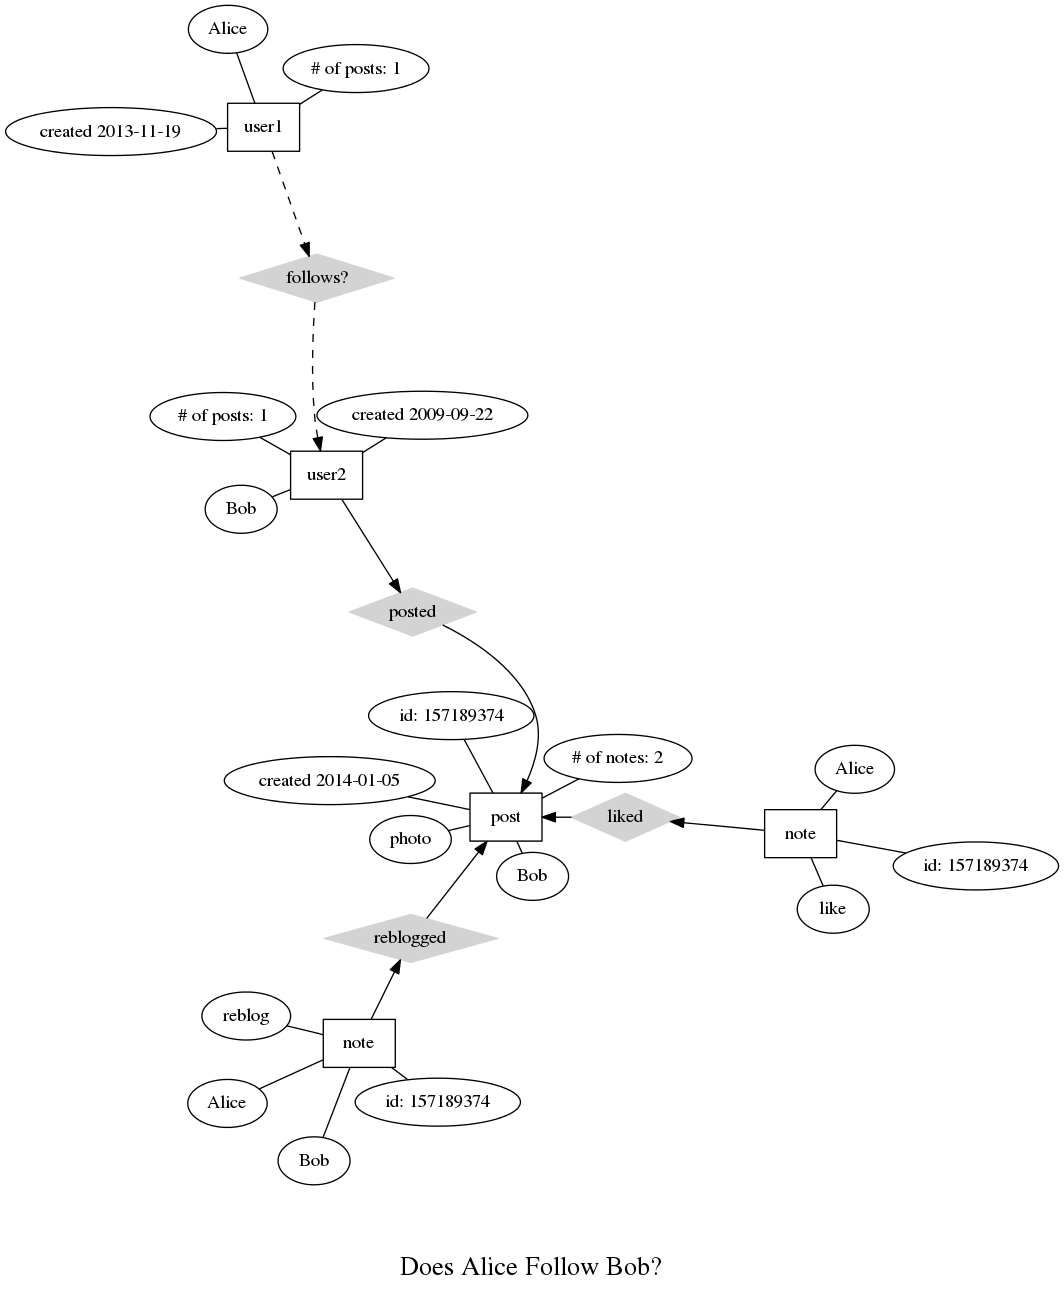
\includegraphics[width=\textwidth]{relations}
 \caption{Here we see a hypothetical relationship between two users}
 \label{fig:relations}
\end{figure*}

For each user, we logged their unique username, the number of posts 
they have contributed to tumblr, and the date they joined. 

For each of those posts, we logged the unique post identifier, the 
date posted, the post type, and the number of notes.

Notes can take two forms: 

user likes content and 

user1, via user2, reblogs content.

We present the following logic as a technique for identifying potential 
links of the form user1 follows user2.

Likes and reblogs on reposts are conserved over all copies.  For likes, 
this means that a like on a reblog of content is indistinguishable from 
a like on the original piece of content itself, or a like on all 
separate instances of the content.
%%% Local Variables: 
%%% mode: latex
%%% TeX-master: "main"
%%% End: 

\section{Results}
\label{sec:-res}
We find that our model of user accuracy is accurate within bounds
%\begin{figure}
%  \input{plots/relations}
%  \caption{}\label{fig:-rel}
%\end{figure}

\begin{figure}[bht]
\centering
 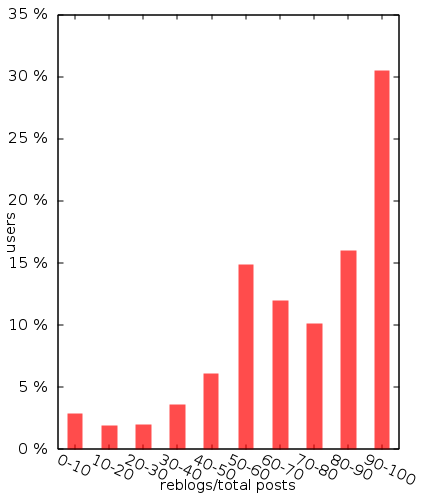
\includegraphics[width=3.5in]{degree}
  \caption{The graph represents the percentage of users, grouped by what percentage of their posts are reblogs}
  \label{fig:-deg}
\end{figure}

This figure indicates that there are very few users that contribute 
primarily original content.  These results indicate 

We find that approximately 15\% of all users generate more original 
content than they repost.  By contrast, 15\% of users post around half 
original content, 30\% repost almost exclusively, and another 40\% or 
so does a considerably higher amount of reblogging than original 
blogging.

We find that the most popular type of post on tumblr is the
\begin{figure}[bht]
\centering
 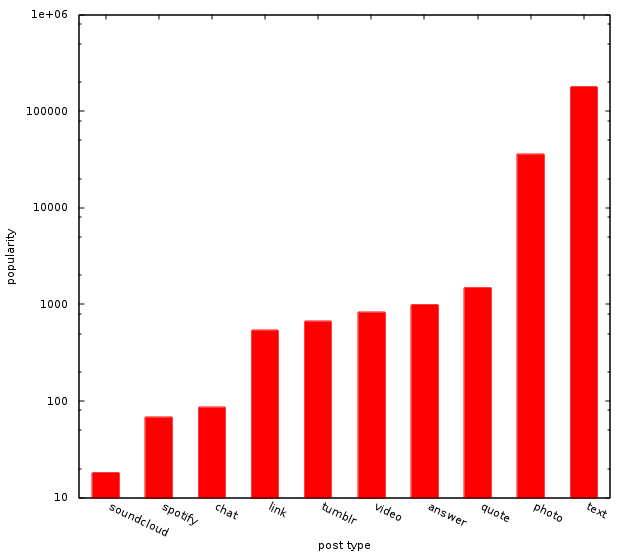
\includegraphics[width=3.5in]{popularity}
  \caption{The graph represents the relative popularity of all surveyed post types.  Note that the graph has a log scale on the y axis}
  \label{fig:-pop}
\end{figure}
This is particularly interesting in light of the 

%%% Local Variables: 
%%% mode: latex
%%% TeX-master: "main"
%%% End: 

\section{Conclusion and Future Work}
\label{sec:-conc}
\subsection{Takeaway}
We speculate that Tumblr, in many ways, reflects the attitudes and 
needs of today's youth.  The anonymity of one's tumbl

\subsection{Future Works}
There are several directions in which this project could be extended, 
given a more liberal timeframe


Although we have operated on a significant subset of Tumblr, we
would like to carry out future studies on a greater breadth of the 
network.  A longer running study could yield a much more robust and 
complete picture of the network.

Early on in the project, we chose not to log post content during the 
running of the crawler.  In part, this was due to the time and space 
constraints imposed by the limited scope of the project, and the power 
of the system available for our research purposes.  In future work, 
time permitting, we could focus further on the textual similarities 
between posts.  Is brevity truly the soul of wit?

In addition, while our current database framework makes it easy to store 
our current data, it is not well-suited to the task of recording tags.  
Tags share a many-to-many relationship with posts, and could be more 
accurately modeled by a more robust object relational mapping.


In addition, we would like to observe the changes in the network from 
different snapshots of Tumblr over a period of months.

We would like to send our inferred follower lists to a number of 
Tumblr users and request some information about the correctness of our 
list, in order to refine our inference method.

As the structure of Tumblr's namespace requires that our crawler be 
bootstrapped from a single hardcoded username, we would like to run our 
study with different starting points.

How many users only like, and are unlikely to do any posting or reblogging?

In future work, we may be interested in seeing how many users not only 
create original content, but also source content from other places.

%%% Local Variables: 
%%% mode: latex
%%% TeX-master: "main"
%%% End: 


\section{Acknowledgments}
We thank Bryan Clement, for lending his expertise in SQL and Python to 
the project as a consultant. We also thank Ellen Klowden, MSW, for 
editorial assistance.

%\small
\bibliography{citations}
\end{document}
